% Options for packages loaded elsewhere
\PassOptionsToPackage{unicode}{hyperref}
\PassOptionsToPackage{hyphens}{url}
%
\documentclass[
  english,
  a4paper]{article}
\usepackage{lmodern}
\usepackage{amsmath}
\usepackage{ifxetex,ifluatex}
\ifnum 0\ifxetex 1\fi\ifluatex 1\fi=0 % if pdftex
  \usepackage[T1]{fontenc}
  \usepackage[utf8]{inputenc}
  \usepackage{textcomp} % provide euro and other symbols
  \usepackage{amssymb}
\else % if luatex or xetex
  \usepackage{unicode-math}
  \defaultfontfeatures{Scale=MatchLowercase}
  \defaultfontfeatures[\rmfamily]{Ligatures=TeX,Scale=1}
\fi
% Use upquote if available, for straight quotes in verbatim environments
\IfFileExists{upquote.sty}{\usepackage{upquote}}{}
\IfFileExists{microtype.sty}{% use microtype if available
  \usepackage[]{microtype}
  \UseMicrotypeSet[protrusion]{basicmath} % disable protrusion for tt fonts
}{}
\makeatletter
\@ifundefined{KOMAClassName}{% if non-KOMA class
  \IfFileExists{parskip.sty}{%
    \usepackage{parskip}
  }{% else
    \setlength{\parindent}{0pt}
    \setlength{\parskip}{6pt plus 2pt minus 1pt}}
}{% if KOMA class
  \KOMAoptions{parskip=half}}
\makeatother
\usepackage{xcolor}
\IfFileExists{xurl.sty}{\usepackage{xurl}}{} % add URL line breaks if available
\IfFileExists{bookmark.sty}{\usepackage{bookmark}}{\usepackage{hyperref}}
\hypersetup{
  pdflang={en},
  hidelinks,
  pdfcreator={LaTeX via pandoc}}
\urlstyle{same} % disable monospaced font for URLs
\usepackage[top=2.4cm, bottom=2.1cm, outer=2cm, inner=4cm, headheight=40pt]{geometry}
\usepackage{color}
\usepackage{fancyvrb}
\newcommand{\VerbBar}{|}
\newcommand{\VERB}{\Verb[commandchars=\\\{\}]}
\DefineVerbatimEnvironment{Highlighting}{Verbatim}{commandchars=\\\{\}}
% Add ',fontsize=\small' for more characters per line
\usepackage{framed}
\definecolor{shadecolor}{RGB}{248,248,248}
\newenvironment{Shaded}{\begin{snugshade}}{\end{snugshade}}
\newcommand{\AlertTok}[1]{\textcolor[rgb]{0.94,0.16,0.16}{#1}}
\newcommand{\AnnotationTok}[1]{\textcolor[rgb]{0.56,0.35,0.01}{\textbf{\textit{#1}}}}
\newcommand{\AttributeTok}[1]{\textcolor[rgb]{0.77,0.63,0.00}{#1}}
\newcommand{\BaseNTok}[1]{\textcolor[rgb]{0.00,0.00,0.81}{#1}}
\newcommand{\BuiltInTok}[1]{#1}
\newcommand{\CharTok}[1]{\textcolor[rgb]{0.31,0.60,0.02}{#1}}
\newcommand{\CommentTok}[1]{\textcolor[rgb]{0.56,0.35,0.01}{\textit{#1}}}
\newcommand{\CommentVarTok}[1]{\textcolor[rgb]{0.56,0.35,0.01}{\textbf{\textit{#1}}}}
\newcommand{\ConstantTok}[1]{\textcolor[rgb]{0.00,0.00,0.00}{#1}}
\newcommand{\ControlFlowTok}[1]{\textcolor[rgb]{0.13,0.29,0.53}{\textbf{#1}}}
\newcommand{\DataTypeTok}[1]{\textcolor[rgb]{0.13,0.29,0.53}{#1}}
\newcommand{\DecValTok}[1]{\textcolor[rgb]{0.00,0.00,0.81}{#1}}
\newcommand{\DocumentationTok}[1]{\textcolor[rgb]{0.56,0.35,0.01}{\textbf{\textit{#1}}}}
\newcommand{\ErrorTok}[1]{\textcolor[rgb]{0.64,0.00,0.00}{\textbf{#1}}}
\newcommand{\ExtensionTok}[1]{#1}
\newcommand{\FloatTok}[1]{\textcolor[rgb]{0.00,0.00,0.81}{#1}}
\newcommand{\FunctionTok}[1]{\textcolor[rgb]{0.00,0.00,0.00}{#1}}
\newcommand{\ImportTok}[1]{#1}
\newcommand{\InformationTok}[1]{\textcolor[rgb]{0.56,0.35,0.01}{\textbf{\textit{#1}}}}
\newcommand{\KeywordTok}[1]{\textcolor[rgb]{0.13,0.29,0.53}{\textbf{#1}}}
\newcommand{\NormalTok}[1]{#1}
\newcommand{\OperatorTok}[1]{\textcolor[rgb]{0.81,0.36,0.00}{\textbf{#1}}}
\newcommand{\OtherTok}[1]{\textcolor[rgb]{0.56,0.35,0.01}{#1}}
\newcommand{\PreprocessorTok}[1]{\textcolor[rgb]{0.56,0.35,0.01}{\textit{#1}}}
\newcommand{\RegionMarkerTok}[1]{#1}
\newcommand{\SpecialCharTok}[1]{\textcolor[rgb]{0.00,0.00,0.00}{#1}}
\newcommand{\SpecialStringTok}[1]{\textcolor[rgb]{0.31,0.60,0.02}{#1}}
\newcommand{\StringTok}[1]{\textcolor[rgb]{0.31,0.60,0.02}{#1}}
\newcommand{\VariableTok}[1]{\textcolor[rgb]{0.00,0.00,0.00}{#1}}
\newcommand{\VerbatimStringTok}[1]{\textcolor[rgb]{0.31,0.60,0.02}{#1}}
\newcommand{\WarningTok}[1]{\textcolor[rgb]{0.56,0.35,0.01}{\textbf{\textit{#1}}}}
\usepackage{longtable,booktabs}
\usepackage{calc} % for calculating minipage widths
% Correct order of tables after \paragraph or \subparagraph
\usepackage{etoolbox}
\makeatletter
\patchcmd\longtable{\par}{\if@noskipsec\mbox{}\fi\par}{}{}
\makeatother
% Allow footnotes in longtable head/foot
\IfFileExists{footnotehyper.sty}{\usepackage{footnotehyper}}{\usepackage{footnote}}
\makesavenoteenv{longtable}
\usepackage{graphicx}
\makeatletter
\def\maxwidth{\ifdim\Gin@nat@width>\linewidth\linewidth\else\Gin@nat@width\fi}
\def\maxheight{\ifdim\Gin@nat@height>\textheight\textheight\else\Gin@nat@height\fi}
\makeatother
% Scale images if necessary, so that they will not overflow the page
% margins by default, and it is still possible to overwrite the defaults
% using explicit options in \includegraphics[width, height, ...]{}
\setkeys{Gin}{width=\maxwidth,height=\maxheight,keepaspectratio}
% Set default figure placement to htbp
\makeatletter
\def\fps@figure{htbp}
\makeatother
\setlength{\emergencystretch}{3em} % prevent overfull lines
\providecommand{\tightlist}{%
  \setlength{\itemsep}{0pt}\setlength{\parskip}{0pt}}
\setcounter{secnumdepth}{5}

    % \documentclass[a4paper]{article}
    % Lang EN = 1, FR = 2
    % \def\Lang{\Sexpr{Lang}} %
    % -- Command to find which language is loaded in babel -- %
    % http://tex.stackexchange.com/questions/287667/ifpackagewith-doesnt-behave-as-i-expected-with-global-options
    \usepackage{xparse}
    \ExplSyntaxOn
    \NewDocumentCommand{\packageoptionsTF}{mmmm}
    {
    \stanton_package_options:nnTF { #1 } { #2 } { #3 } { #4 }
    }

    \cs_new_protected:Nn \stanton_package_options:nnTF
    {
    \clist_map_inline:nn { #2 }
    {
    \clist_if_in:cnTF { opt@#1.sty } { ##1 }
    { #3 } % it is a local option
    {
      \clist_if_in:cnTF { @classoptionslist } { ##1 }
        { #3 } % it is a global option
          { #4 }
          }
        }
      }
      \ExplSyntaxOff

      % -- Define a variable depending on language -- %
        \newcommand{\Lang}{0}

      \makeatletter
      \@ifpackageloaded{babel}{
        \packageoptionsTF{babel}{english}{%
          \renewcommand{\Lang}{1}% english
        }{%
          \renewcommand{\Lang}{2}% french
        }
      }{}
      \makeatother

      % -- Define specific lateX options depending on language -- %
        \ifnum\Lang = 1
      % \usepackage[english]{babel}
      \usepackage{enumitem}
      \setlist{itemsep = 0pt}
      \setlist{topsep = 0pt}
      \fi
      \ifnum\Lang = 2
      % \usepackage[french]{babel}
      \fi

      % --
     % \input{/mnt/Data/ThinkR/Gitlab/vignette-thinkr/latex/MiseEnPageRmd.tex")}
       
% === BEGIN OF pdf_layout === %
\usepackage[utf8]{inputenc}
\usepackage[T1]{fontenc}
\usepackage{amsmath}
%\usepackage{amssymb,amsfonts,textcomp}
\usepackage{color}
\usepackage{array}
\usepackage{hhline}
%\usepackage[linktocpage=true]{hyperref} % to have only number clickable in toc
\hypersetup{linktocpage=true, colorlinks=true, linkcolor=[RGB]{190,3,2}, citecolor=[RGB]{190,3,2}, filecolor=[RGB]{190,3,2}, urlcolor=[RGB]{190,3,2}}
%\usepackage[pdftex]{graphicx}
\usepackage{tikz}
%\usepackage{float} % To force figure to be placed where I want with H
% do not use float as it changes space between figures and their caption.
% Better use [!h] option for figures
\usepackage[normalem]{ulem} % to underline text on multiple lines

\renewcommand{\emph}[1]{\textit{#1}}

\usepackage{lmodern} % For higher definition fonts
\usepackage[font = footnotesize, labelfont = bf, margin = 1cm]{caption} %name=Fig.

% Text styles
\newcommand\majorstylecolor[1]{\textcolor[RGB]{190,3,2}{#1}}
\newcommand\urlstylecolor[1]{\textcolor[RGB]{190,3,2}{#1}}
\newcommand\Greytext[1]{\textcolor[RGB]{75,75,75}{#1}}
\newcommand\LightGrey[1]{\textcolor[RGB]{173,169,174}{#1}}
\newcommand\OtherGrey[1]{\textcolor[RGB]{200,200,200}{#1}}


% List styles
%\newcommand\liststyleWWviiiNumii{%
%\renewcommand\labelitemi{{\textbullet}}
%\renewcommand\labelitemii{{\textbullet}}
%\renewcommand\labelitemiii{{\textbullet}}
%\renewcommand\labelitemiv{{\textbullet}}
%}

\AtBeginDocument{
\def\labelitemi{$\bullet$}%
\def\labelitemii{$\circ$}%
\def\labelitemiii{$-$}%
\def\labelitemiv{$-$}%
}

% FIGURES
% \graphicspath{{/mnt/Data/Formation_SIG-et-R/00_Original_TD_support/img_QGIS/}{/mnt/Data/Formation_SIG-et-R/00_Original_TD_support/figureR/}{/mnt/Data/Formation_SIG-et-R/00_Original_TD_support/Figures_Pres/}{/mnt/Data/autoentrepreneur/Presentation_Produits/SRochettePresentation-img/}}

%\setlength{\abovecaptionskip}{5pt}
%\setlength{\belowcaptionskip}{10pt}


% DIMENSIONS - MARGINS
% \usepackage[top=2.4cm, bottom=2.1cm, outer=2cm, inner=4cm, headheight=40pt]{geometry} %heightrounded
%\setlength\hoffset{0cm}
%\setlength\voffset{0cm}
\setlength\topmargin{-2cm}
%\setlength\headheight{2cm}
\setlength\headsep{0.50cm}
%\setlength\textheight{25.7cm}
\setlength\footskip{1.1cm}
\setlength{\parindent}{0em}
%\setlength{\parskip}{0em}
\setlength\belowcaptionskip{5pt}
\setlength\abovecaptionskip{8pt}
%\let\oldfigure\figure
%\let\oldtable\table
%\def\figure{\setlength\abovecaptionskip{5pt}\oldfigure}
%\def\table{\setlength\belowcaptionskip{1cm}\oldtable}
%\usepackage{caption} %[font = small]
%\setlength{\abovecaptionskip}{10pt plus 5pt minus 5pt}
%\captionsetup[table]{skip = 10pt}
%\captionsetup[figure]{skip = 10pt}
%\setlength\longindentation 0.60\textwidth

% \usepackage{lastpage} % to calculate number of pages to put in footer
\usepackage{pageslts}

% ----------
% BACKGROUND
% ----------
\usepackage{eso-pic}
\newcommand\BackgroundPic{%
\put(0,0){%
\parbox[b][\paperheight]{\paperwidth}{%
\vfill
\centering

\includegraphics[width=\paperwidth,height=\paperheight]{Background_deepred_topdown.png}%
\vfill
}}}
\newcommand\BackgroundPicTitle{%
\put(0,0){%
\parbox[b][\paperheight]{\paperwidth}{%
\vfill
\centering

\includegraphics[width=\paperwidth,height=\paperheight]{Background_Title_deepred_2.png}%
\vfill
}}}

%...and this immediately after \begin{document}:
%\AddToShipoutPicture*{\BackgroundPic}
%The * will make sure that the background picture will only be put on one page.
%If you wish to use the picture on multiple pages, skip the *:
%\AddToShipoutPicture{\BackgroundPic}
%Then use this command to stop using the background picture:
%\ClearShipoutPicture

% === END OF pdf_layout === %
    
       % \input{/mnt/Data/ThinkR/Gitlab/vignette-thinkr/latex/MiseEnFormeTitreFormationRmd.tex")}
       
  % ----------
% BEGIN pdf_sections
  % ----------
% MISE EN FORME DES TITRES
       % ----------
       %\renewcommand{\thesection}{\arabic{section}}
       %\renewcommand{\thesubsection}{\arabic{section}.\arabic{subsection}}
       %\renewcommand{\thesubsubsection}{\arabic{section}.\arabic{subsection}.\arabic{subsubsection}}

       %% Provide a definition to \subparagraph to keep titlesec happy
       \let\subparagraph\oldsubparagraph
       \let\paragraph\oldparagraph
       %% Load titlesec
       %\usepackage[compact]{titlesec}
       \usepackage{titlesec}
       %% Revert \subparagraph to the Rmd definition
       % Redefines (sub)paragraphs to behave more like sections
       \ifx\paragraph\undefined\else
       \let\oldparagraph\paragraph
       \renewcommand{\paragraph}[1]{\oldparagraph{#1}\mbox{}}
       \fi
       \ifx\subparagraph\undefined\else
       \let\oldsubparagraph\subparagraph
       \renewcommand{\subparagraph}[1]{\oldsubparagraph{#1}\mbox{}}
       \fi


       %\titleformat{(command)}[(shape)]{(format)}{(label)}{(sep)}{(before)}[(after)]
       \titleformat{\section}%
       [block]% style du titre (block, hang, display, runin, leftmargin, drop, wrap)
       {\Large\color[RGB]{0,153,255}}%changement de fonte commun au numero et au titre
       {\thesection.}% specification du numero
       {1em}% 1em espace entre le numero et le titre
       {}% changement de fonte du titre

       \titleformat{\subsection}%
       [block]% style du titre (block, hang, display, runin, leftmargin, drop, wrap)
       {\large\bfseries} %\itshape {\Large\bfseries\color[RGB]{0,153,255}}%changement de fonte commun au numero et au titre
       {\thesubsection.}% specification du numero
       {1em}% {1em}% espace entre le numero et le titre
       {}% changement de fonte du titre

       %\titlespacing*{(command)}{(left)}{(beforesep)}{(aftersep)}[(right)]
       \titlespacing*{\section}{0em}{*4}{*1}

       % A break for each new section with figures printed before new section
       % \newcommand{\sectionbreak}{\clearpage}
       % \newcommand{\sectionbreak}{\clearpage\phantomsection} % if hyperref loaded before titlesec

       % Title numbering depth
       \setcounter{secnumdepth}{3}
       % Table of content depth
       \setcounter{tocdepth}{3}
       \renewcommand\contentsname{Content} % toc title

        % Keep color format
        \newcommand\sectionstylecolor[1]{\textcolor[RGB]{0,153,255}{#1}}


       % -----------
       % MISE EN FORME TEXTES SPECIAUX
       % -----------
       % Additionnal Text colors
       \usepackage{xcolor}
       \definecolor{backcolor}{RGB}{235, 235, 235}

       \newcommand{\mybox}[1]{\par\noindent\colorbox{backcolor}
       {\parbox{\dimexpr\textwidth-2\fboxsep\relax}{#1}}}

       \newcommand{\keyword}[1]{\textcolor{red!60!black}{#1}}
       \newcommand{\advert}[1]{\textit{\textcolor{orange!80!black}{#1}}}
       \newcommand{\exo}[1]{\textit{\textcolor{green!80!black}{#1}}}
       %\newcommand{\codecommand}[1]{\par\noindent\colorbox{backcolor}{\texttt{#1}}}
       %\newcommand{\menucommand}[1]{\par\fontfamily{pcr}\fontsize{12}{12}\selectfont\color{red}\noindent\colorbox{shadecolor}{\textit{#1}}}{\par}
       \newcommand{\menucommand}[1]{\textit{\textcolor{blue!80!black}{#1}}}
       \newcommand{\codecommand}[1]{\texttt{\colorbox{backcolor}{#1}}}

       \newenvironment{important}{\par\color{black!80!green}\itshape}{\par}

       \newsavebox{\selvestebox}
       \newenvironment{redbox}
       {
       \begin{lrbox}{\selvestebox}%
       \begin{minipage}{\dimexpr\columnwidth-2\fboxsep\relax}}
       {\end{minipage}\end{lrbox}%
       \colorbox[HTML]{FF7F7F}{\usebox{\selvestebox}}
       }

       % \newsavebox{\selvestebox}
       \newenvironment{codebox}{
       \begin{lrbox}{\selvestebox}%
       }{
       \end{lrbox}%
       \colorbox{backcolor}{\usebox{\selvestebox}}
       }

       % - source: http://tex.stackexchange.com/questions/82028/how-do-i-create-a-variant-of-the-snugshade-box-from-the-framed-package-to-wrap-m
       \newenvironment{blueShaded}[1][D6E8F5]{
       \definecolor{shadecolor}{HTML}{#1}%
       \begin{snugshade}%
       }{%
       \end{snugshade}%
       }

       % -- command for pandoc trick with \begin and \end -- %
       \newcommand{\nopandoc}[1]{#1}

       % ----------
       % Pour justifier le texte apres un alignement a gauche
       % Utile pour le texte en caractere tt qui ne se coupe pas
       % ----------
       \usepackage{ragged2e}

  % ----------
% END pdf_sections
  % ----------
   
      % \input{/mnt/Data/ThinkR/Gitlab/vignette-thinkr/latex/MiseEnFormeTitreFormationRmd_NoSectionBreak.tex}

       
     % ---------------
% HEADER / FOOTER
     % ---------------
     \usepackage{fancyhdr}
     \pagestyle{fancy}
     %\fancyhf{}
     \fancyhead[L]{
     \hspace{-1cm}\LARGE{\textbf{\href{https://rtask.thinkr.fr}{\majorstylecolor{Tonico Traning}}}}\\
     \hspace{-1cm}\normalsize{\Greytext{R report}}\\
     %\normalsize{\href{url:https://statnmap.com/}{\majorstylecolor{http://statnmap.com/}}}
     }
     \fancyhead[R]{\Greytext{\textit{Created on \today}\hspace{-1cm}}}
     %
     \fancyfoot[L]{\hspace{-1cm}\Greytext{TT}}
     \fancyfoot[C]{\href{mailto:sebastien@thinkr.fr}{sebastien@thinkr.fr}}
     \fancyfoot[R]{\Greytext{\thepage\ / \pageref*{LastPage}\hspace{-1cm}}}
     %\cfoot{Page \thepage\ (\theCurrentPage) of \lastpageref{LastPages}}
     \renewcommand{\headrulewidth}{0pt}
     \renewcommand{\footrulewidth}{0pt}
     %\fancyheadoffset{length}

      

      % -- Graphic path -- %
      % \graphicspath{{"/img/"}}

      \setcounter{section}{0} % Value for first section
       
\hypersetup{pdfauthor=TT, pdftitle=general report, pdfsubject=general report, pdfkeywords=R, pdfcreator=pdflatex}

         %----------------------------------------------------------------------------------------
         % TITLE PAGE
         %----------------------------------------------------------------------------------------

          % The original for this is the title page for Gentle Madness by Nicholas Basbanes [Bas95]

         \newcommand*{\titleGM}{\begingroup % Create the command for including the title page in the document
         \hbox{ % Horizontal box
         %\hspace*{0.2\textwidth} % Whitespace to the left of the title page
         %\hspace*{0.2\textwidth}
         \OtherGrey{\rule{1pt}{\textheight}} % Vertical line
         \hspace*{0.05\textwidth} % Whitespace between the vertical line and title page text
         \parbox[b]{0.75\textwidth}{ % Paragraph box which restricts text to less than the width of the page

         {\noindent\Huge\bfseries\majorstylecolor{general report}}\\[2\baselineskip] % Title
         {\large{a sport nutrition template}}\\[4\baselineskip] % Tagline or further description
         {\Large \textsc{TT, Tonico Traning}} % Author name

         \vspace{0.5\textheight} % Whitespace between the title block and the publisher
         {\noindent \href{https://rtask.thinkr.fr}{Tonico Traning}}\\[\baselineskip] % Publisher and logo
         }}
         \endgroup}

         \AtBeginDocument{\let\maketitle\relax}
          
\ifxetex
  % Load polyglossia as late as possible: uses bidi with RTL langages (e.g. Hebrew, Arabic)
  \usepackage{polyglossia}
  \setmainlanguage[]{english}
\else
  \usepackage[shorthands=off,main=english]{babel}
\fi
\ifluatex
  \usepackage{selnolig}  % disable illegal ligatures
\fi

\author{}
\date{\vspace{-2.5em}}

\begin{document}

\pagenumbering{arabic}

%\bigskip
%\medskip

%\begin{center}
%\href{url:http://statnmap.com}{\textstyleInternetlink{\huge{Modelling distribution of species in the Bay of Biscay}}}\\
%\large{Sébastien Rochette}\\
%\end{center}
\setcounter{page}{0}
\pagestyle{empty} % Removes page numbers
\AddToShipoutPicture{\BackgroundPicTitle}

\titleGM

\pagebreak
\pagestyle{fancy}
% \clearpage\setcounter{page}{1}\pagestyle{Standard}
\AddToShipoutPicture{\BackgroundPic}

{
\setcounter{tocdepth}{2}
\tableofcontents
}
\hypertarget{section-1}{%
\section{Section 1}\label{section-1}}

\hypertarget{general-advices-to-client-na}{%
\subsection{General Advices to client: NA}\label{general-advices-to-client-na}}

\hypertarget{goal}{%
\subsection{Goal:}\label{goal}}

NA

\hypertarget{remeber}{%
\subsection{Remeber:}\label{remeber}}

NA

This is an R Markdown document. Markdown is a simple formatting syntax for authoring HTML, PDF, and MS Word documents. For more details on using R Markdown see \url{http://rmarkdown.rstudio.com}.

When you click the \textbf{Knit} button a document will be generated that includes both content as well as the output of any embedded R code chunks within the document. You can embed an R code chunk like this:

\begin{Shaded}
\begin{Highlighting}[]
\FunctionTok{summary}\NormalTok{(cars)}
\end{Highlighting}
\end{Shaded}

\begin{verbatim}
##      speed           dist       
##  Min.   : 4.0   Min.   :  2.00  
##  1st Qu.:12.0   1st Qu.: 26.00  
##  Median :15.0   Median : 36.00  
##  Mean   :15.4   Mean   : 42.98  
##  3rd Qu.:19.0   3rd Qu.: 56.00  
##  Max.   :25.0   Max.   :120.00
\end{verbatim}

\hypertarget{including-plots}{%
\subsection{Including Plots}\label{including-plots}}

You can also embed plots with reference and caption as in Fig. \ref{fig:pressure}.



\begin{figure}
\centering
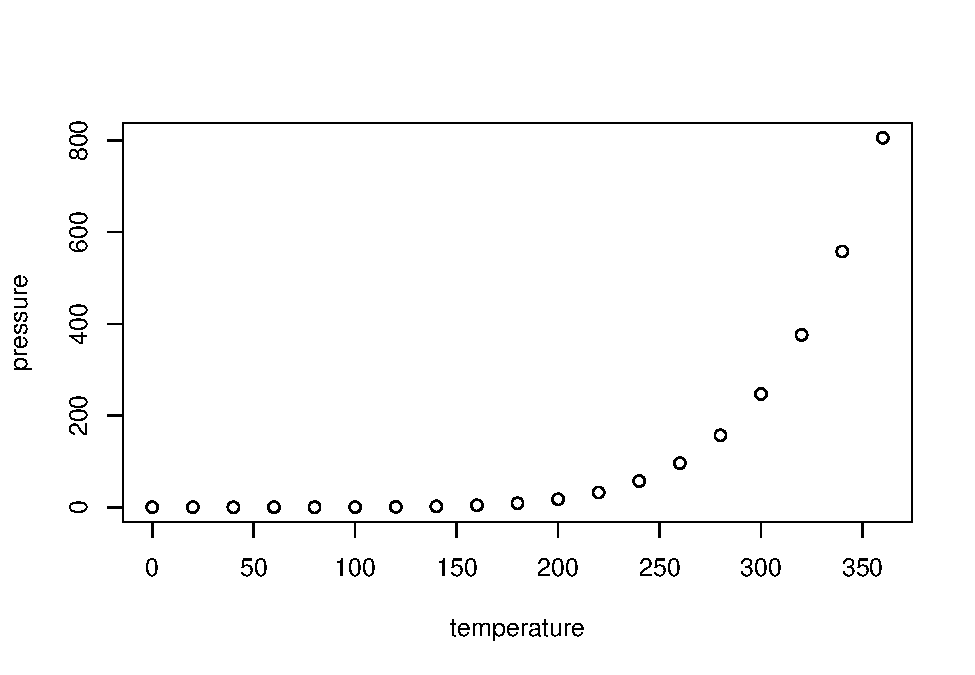
\includegraphics{reportpdf_files/figure-latex/pressure-1.pdf}
\caption{\label{fig:pressure}Pressure of cars}
\end{figure}

Note that the \texttt{echo\ =\ FALSE} parameter was added to the code chunk to prevent printing of the R code that generated the plot.

\hypertarget{a-few-extra}{%
\subsection{A few extra}\label{a-few-extra}}

\majorstylecolor{\textbackslash majorstylecolor\{Text with same color as main title\}}  
\urlstylecolor{\textbackslash urlstylecolor\{Text with same color as url\}}  
\sectionstylecolor{\textbackslash sectionstylecolor\{Text with same color as section title\}}  
\keyword{\textbackslash keyword\{To put some word in darkred\}}  
\advert{\textbackslash advert\{To put some words in orange and italic\}}

\end{document}
